\documentclass {article}
\usepackage{amsmath,graphicx,listings,xcolor,hyperref,float}
\graphicspath{ {imagenes/} }


\begin{document}
\title{Manual de Uso Practica 2}
\maketitle
\begin{center}
  
\includegraphics[scale=0.2]{gnu}\\
  \vspace{3cm}
  \textbf{Eduard Joel Ostos Castro}\\
  \textbf{Andres Felipe Sanchez Ladino}\\ 
  \textbf{Tania Julieth Araque Dueñas}\\ 
\end{center}

\newpage
\lstset{
  backgroundcolor=\color{lightgray},
  basicstyle=\footnotesize,
  breaklines=true,
  captionpos=b,
  tabsize=2
}

\section{Del lado del servidor}:w
El servidor puede iniciarse en un computador de manera local, se tendrá la IP local, localhost (en la mayoría de los casos), entonces luego para iniciar el servidor se ejecuta el programa, con ./server seguido de algún puerto, ej:
\begin{lstlisting}{language=C}
./server 49152
\end{lstlisting}

No es necesario colocar una IP al servidor, este la encontrará de manera automatica.
\section{Del lado del cliente}
\subsection{Conectarnos al servidor}
\begin{enumerate}
  \item{\textbf{Servidor en modo local}}
    Para esta conexión solo resta iniciar el server como ya se vió en el item anterior, y el cliente se inicializa de esta forma:
    \begin{lstlisting}{language=C}
      ./client localhost 49152
    \end{lstlisting}
    \textbf{No olvidar, la IP es el primer parametro, el segundo es el puerto, el cual debe concordar con el puerto al que se conectó el server.}
    
  \item{\textbf{Servidor en modo online}}
Para una satisfactoria conexión al servidor antes se le proveerá la dirección IP publica en la que se aloja el servidor, luego deberá iniciar el cliente, en la carpeta en la que tiene cliente.c deberá hace make, el cual, con ayuda del makefile,compilará todo lo necesario para que funcione todo el programa, entonces, iniciará el cliente con el archivo ejecutable, los parametros son similares a los del punto anterior, sin embargo, el primero cambiará, deberá colocar la IP publica en la que se aloja su servidor.
\end{enumerate}

\subsection{Peticiones al servidor}
Estas se realizaran de la misma manera, el cliente hará consultas y el servidor les devolverá respuestas, el esquema del cliente se ve así:\\

  \begin{center}
    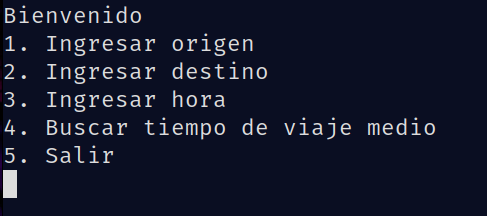
\includegraphics[scale=0.2]{cliente}
  \end{center}


\bibliographystyle{plain}
\bibliography{bibliografia}

\end{document}


